\documentclass[tikz,border=5mm]{standalone}
\usetikzlibrary{decorations.markings}

\begin{document}
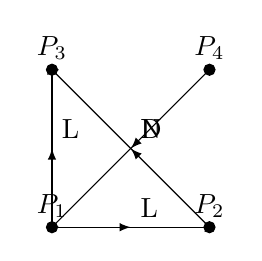
\begin{tikzpicture}
    \tikzset{
        myarrow/.style={
            postaction={
                decorate,
                decoration={
                    markings,
                    mark=at position #1 with {\arrow{latex}},
                },
            },
        },
    }

    % Vertices
    \draw[fill=black] (0, 0) circle (2pt) node[above] {$P_1$};
    \draw[fill=black] (2, 0) circle (2pt) node[above] {$P_2$};
    \draw[fill=black] (0, 2) circle (2pt) node[above] {$P_3$};
    \draw[fill=black] (2, 2) circle (2pt) node[above] {$P_4$};

    % Arcs
    \draw[->, myarrow=.5] (0,0) -- node[midway, above right] {L}  (2,0);
    \draw[->, myarrow=.5] (0,0) -- node[midway, above right] {L}  (0,2);
    \draw[->, myarrow=.5] (2,2) -- node[midway, above right] {N}  (0,0);
    \draw[->, myarrow=.5] (2,0) -- node[midway, above right] {D}  (0,2);
\end{tikzpicture}
\end{document}
